\documentclass[main.tex]{subfiles}

%\externalcitedocument{bibfile}

\begin{document}

\section{IceCube Upgrade}

Introduce physics goals of IceCube upgrade, show some plots that compare old v new event displays. 

\begin{figure}
    \centering
    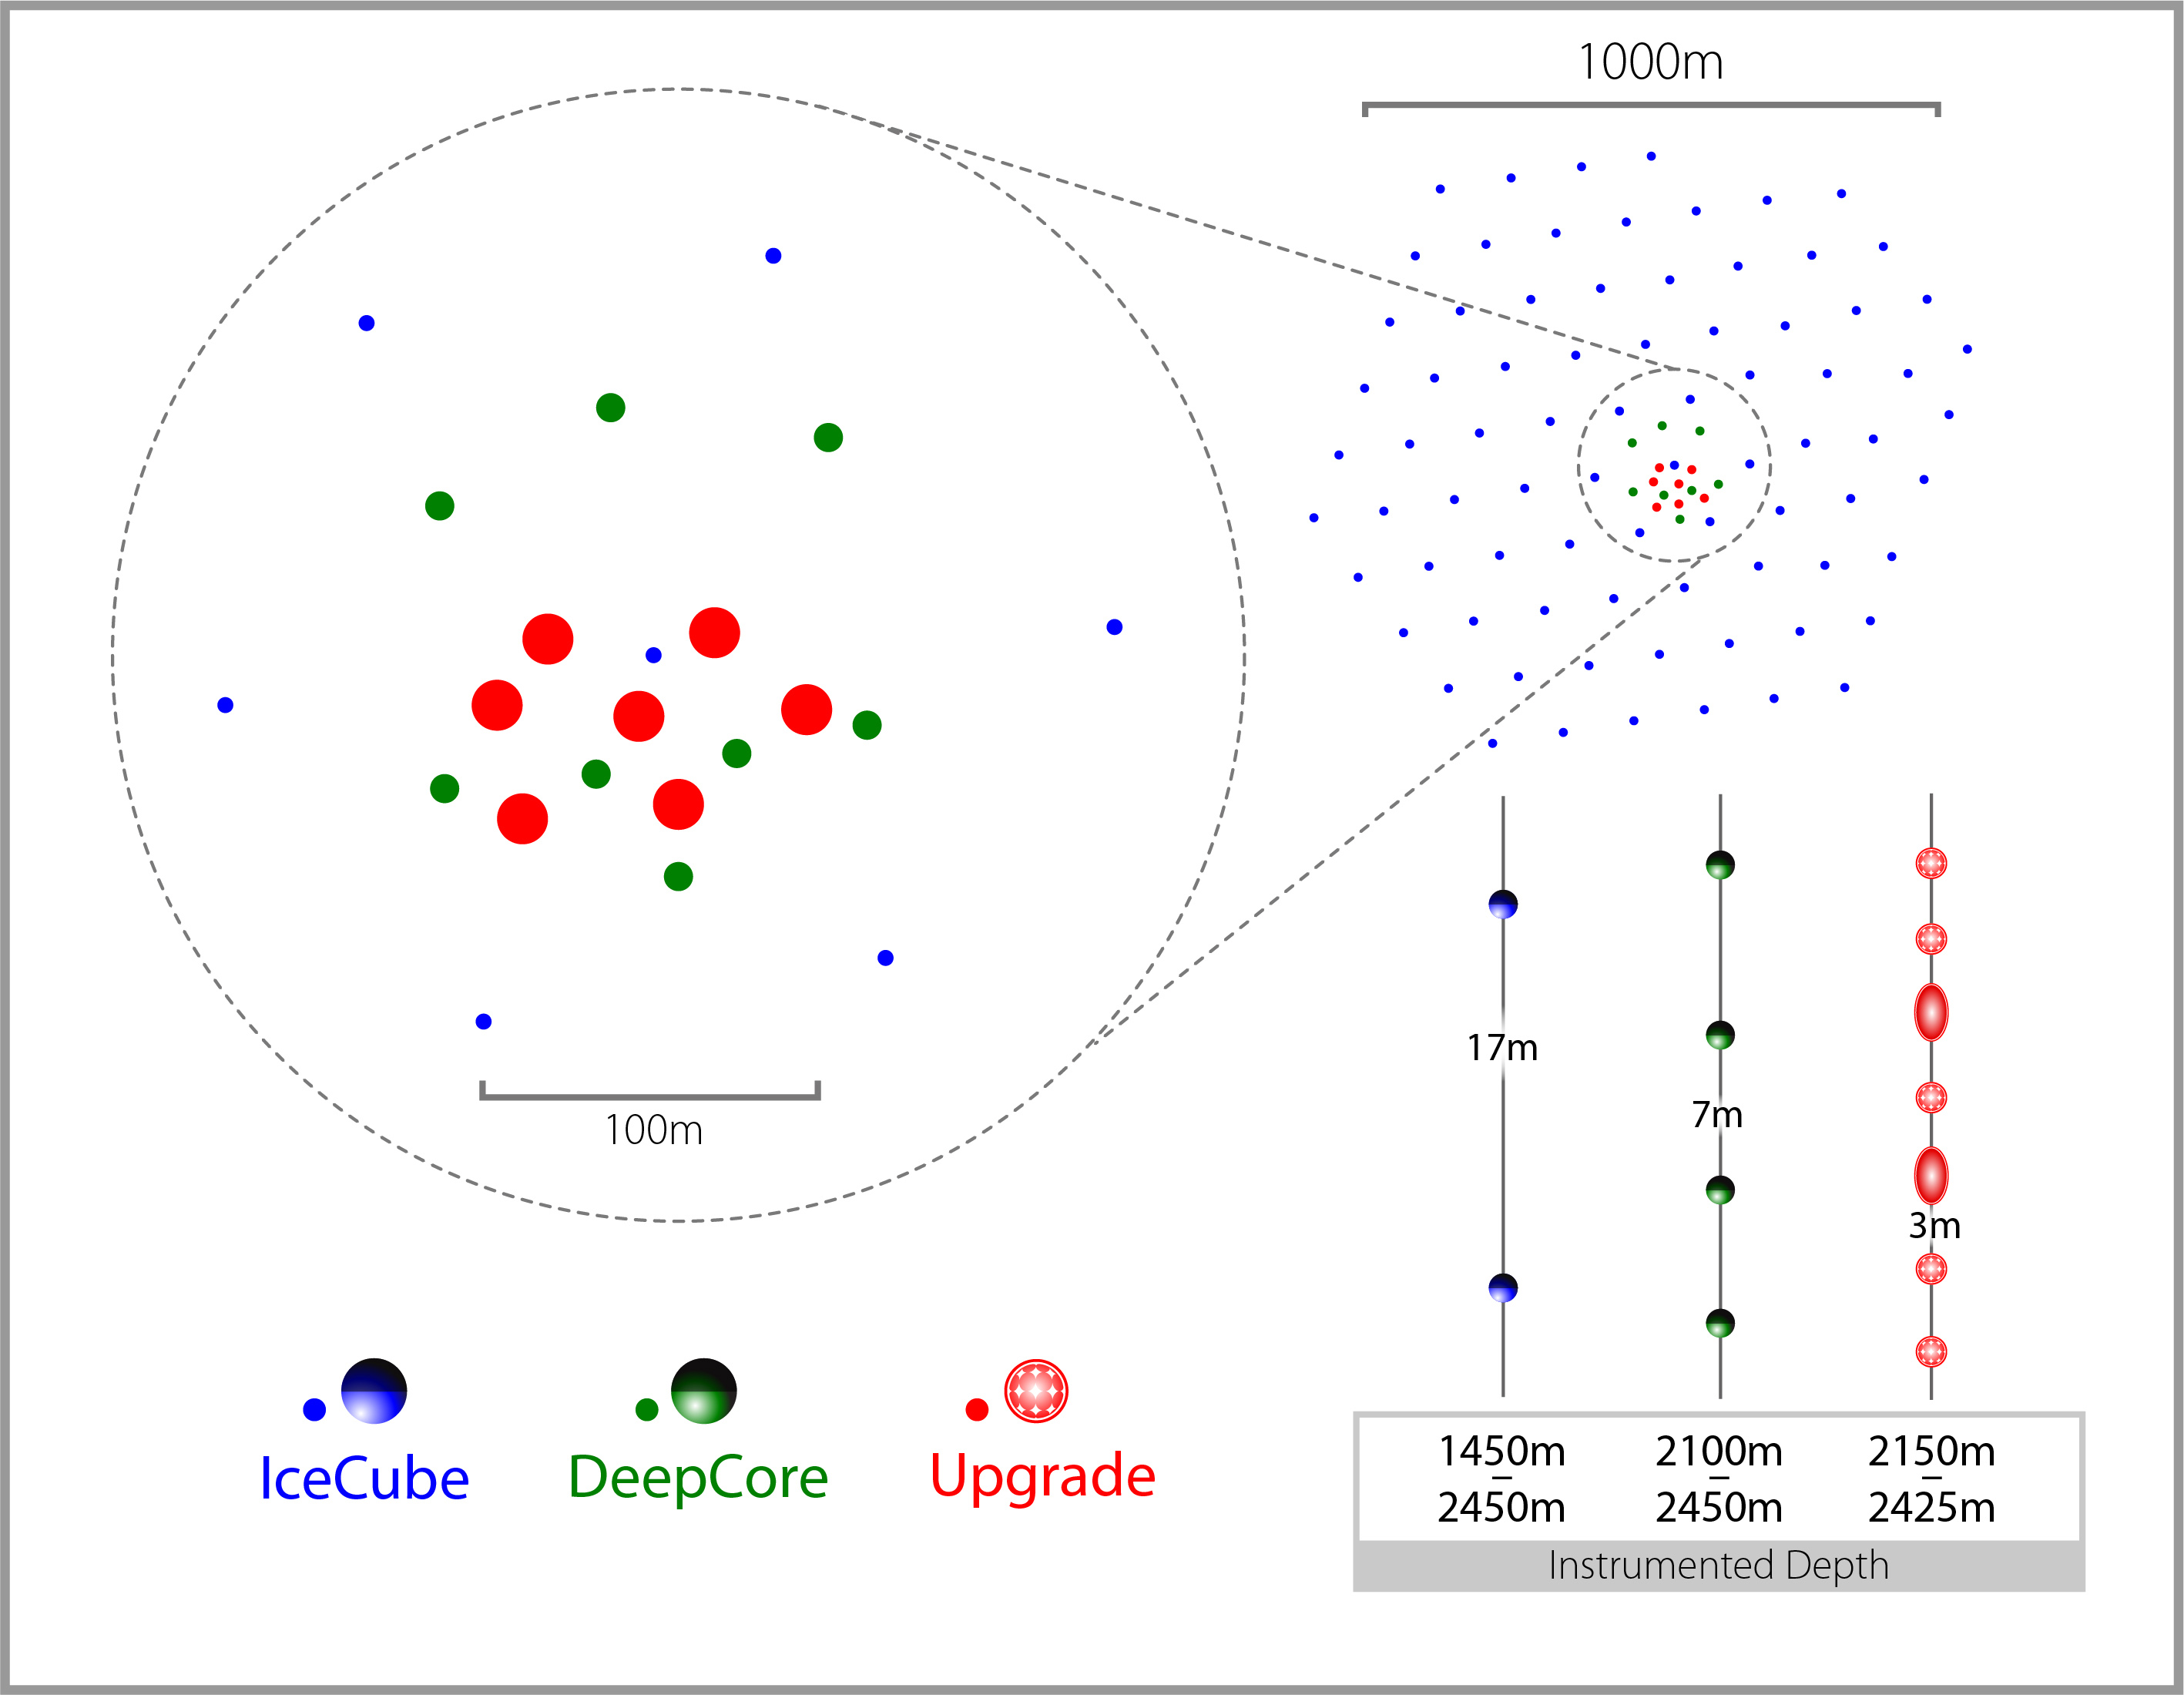
\includegraphics[width=\linewidth]{figures/ICUpgradeLayout_V4b.jpg}
    \caption{A top-down view of the planned installation locations of IceCube Upgrade strings relative to existing IceCube and DeepCore strings.}
    \label{fig:degglayout}
\end{figure}

\section{IceCube D-Eggs}

The ``Dual optical sensors in an Ellipsoid Glass for Gen2,'' or DEgg, is a new module designed for future extensions of IceCube. \ref{fig:degglayout}

DOS-Eggis 

\section{Final Acceptance Testing (FAT) of D-Eggs}

For testing, D-Eggs are tested in batches of fifteen plus one reference D-Egg. 
They are lifted into a freezer, capable of reaching temperatures as low as negative sixty degrees Celcius, and placed into light-sealed boxes in order to isolate individual D-Eggs from one another. 
Optical fibers and insulated cables are routed into the freezer to provide communications, power, and light sources to each D-Egg. 

IceBoot sessions are then established with the D-Eggs and we begin taking measurements. 
Measurements are taken on a consistent basis as the freezer is brought to negative forty degrees Celcius, then up to negative twenty again, back down to negative forty, and then returned to room temperature (approximately twenty degrees Celcius). 

\begin{figure}
    \centering
    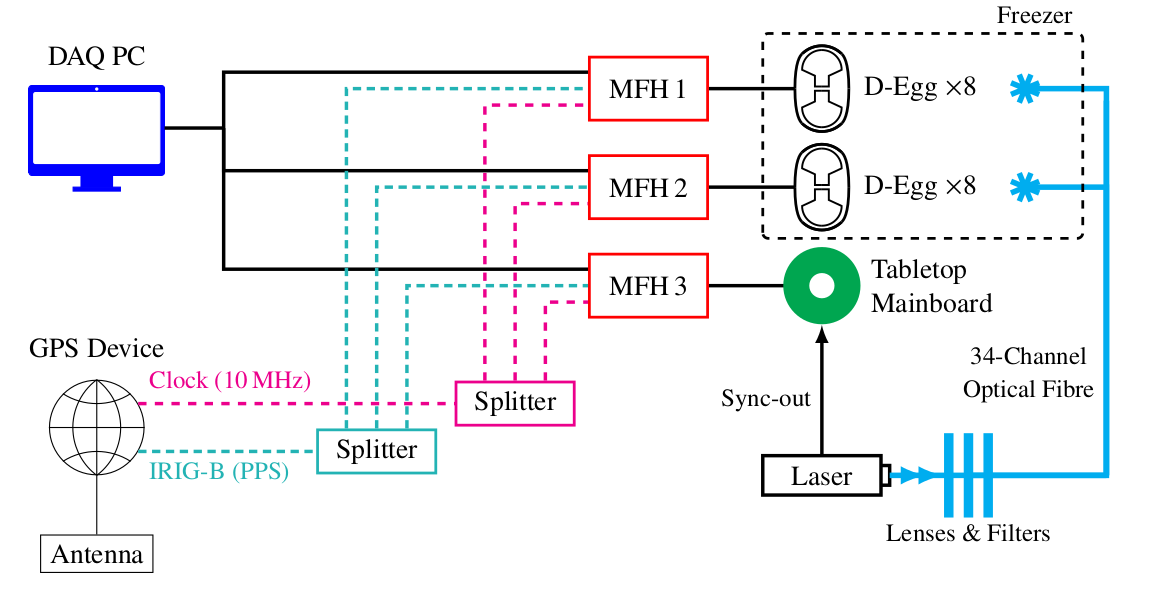
\includegraphics[width=\linewidth]{figures/fat_layout.png}
    \caption{A schematic layout of the FAT layout. }
    \label{fig:fatscheme}
\end{figure}

The block-diagram FAT facility is shown in Figure~\ref{fig:fatscheme}. 
A dedicated data aquisition (DAQ) computer, or DAQ PC, is used to communicate with D-Eggs via two Mini FieldHubs (MFHs); these are simplified versions of the hardware used on-site at the South Pole to communicate with in-ice DOMs. 
A third MFH is used to synchronize timing between a pulsed laser source and the other two MFHs. 
The light source used is a Hamamatsu PLP-10 C10196 with a 400 nm picosecond laser diode head M10306.
Two programmable filter wheels with six distinct neutral density filters are used to attenuate the laser light by discrete amounts. 
The laser light is carried through optical fiber to expose both the top and bottom PMTs of each D-Egg.
This allows for the characterization of the gain of each D-Egg PMT at light levels ranging from low-occupancy SPE to more than 200 SPE levels. 

A 10 MHz clock and the IRIB-B GPS time signals are split and fed into each of the MFHs to synchronize their internal clocks to UTC.
This allows for conversion of the internal D-Egg timestamps to UTC using the standard IceCube Reciprocal Active Pulsing (RAPCal) method~\cite{ABBASI2009294}.


\subsection{Quick Monitoring}

\subsection{Detailed Monitoring}

Once a target temperature is met and the high-voltage, necessary for a gain of 1e7, for the D-Egg PMTs is found, a measurements are carried out to test the stability of the gain and high-voltage of the D-Eggs' PMTs over time. 

\subsection{Analyses}

Once the measurements are taken, data are transfered from the local DAQ PC to the grappa server system in Chiba. Several analyses are then performed. 
First, a fit is performed to check for a linear relationship between gain and the set PMT high-voltage.  
The dark-rate of the PMTs is then 

\end{document}